% ─────────────────────────────────────────────────────────────────
\section{Results and Comparison}
\label{sec:results}
% ─────────────────────────────────────────────────────────────────

\subsection{Main Results Table}

Table~\ref{tab:main_results} summarises all runs in this study alongside
three SHREC\,25 external entries including the RIConv2 method of Barisin
et al.~\cite{riconv2}.
All HierGIN metrics use the proper 88-class evaluation protocol
(Section~\ref{sec:eval_protocol}).
RIConv2 metrics are recomputed from their published prediction CSVs under
the same 88-class protocol.
Both methods are evaluated on the 88 classes that have test proteins in the
official SHREC\,25 test set; 11 of the 99 families have no test proteins
(including classes 97 and 98) and are therefore excluded from all
macro-averaged metrics.

\begin{table}[ht]
  \centering
  \caption{Test set performance --- all methods (88-class macro-F1 protocol).
           \textbf{Bold}: best value per metric column.
           $\ddagger$~Injection runs use 14D (global norm) features.
           RIConv2 metrics recomputed from published prediction CSVs.}
  \label{tab:main_results}
  \setlength{\tabcolsep}{4.5pt}
  \begin{tabular}{llrrrr}
    \toprule
    \textbf{Method} & \textbf{Features}
      & \textbf{Acc} & \textbf{Bal.Acc} & \textbf{Macro-F1} & \textbf{Wtd-F1} \\
    \midrule
    \multicolumn{6}{l}{\textit{External baselines (other SHREC\,25 entries)}} \\
    \quad Flat GIN (h512, 6L)         & 4D                  & ---   & ---   & 0.640 & ---   \\
    \quad Mamba3D~\cite{mamba3d}      & point cloud         & ---   & 0.662 & 0.672 & 0.825 \\
    \quad PointMamba~\cite{pointmamba}& point cloud         & ---   & 0.714 & 0.720 & 0.872 \\
    \quad RIConv2 RUN1~\cite{riconv2} & xyz + normals only  & 0.914 & 0.813 & 0.838 & 0.910 \\
    \quad \textbf{RIConv2 RUN2}~\cite{riconv2} & xyz + normals + Potential & \textbf{0.929} & \textbf{0.828} & \textbf{0.854} & \textbf{0.925} \\
    \midrule
    \multicolumn{6}{l}{\textit{HierGIN --- feature ablation (standard GIN backbone)}} \\
    \quad HierGIN 6D                  & xyz + normals        & 0.783 & 0.612 & 0.619 & 0.760 \\
    \quad HierGIN 7D (no Pot)         & no Potential         & 0.808 & 0.681 & 0.680 & 0.799 \\
    \quad HierGIN 4D                  & xyz + Potential      & 0.845 & 0.796 & 0.784 & 0.843 \\
    \quad HierGIN 7D (no NormPot)     & no NormalPotential   & 0.849 & 0.797 & 0.790 & 0.848 \\
    \quad HierGIN 8D                  & all 8 features       & 0.853 & 0.800 & 0.798 & 0.853 \\
    \midrule
    \multicolumn{6}{l}{\textit{HierGIN --- enriched features (14D = 8D + 6 geometric)}} \\
    \quad HierGIN 14D (z-scored)      & per-protein z-score  & 0.838 & 0.757 & 0.752 & 0.837 \\
    \quad HierGIN 14D (global norm)   & global norm          & 0.865 & 0.812 & \textbf{0.808} & 0.862 \\
    \midrule
    \multicolumn{6}{l}{\textit{HierGIN --- rotation-invariant backbone (RI-GIN)}} \\
    \quad HierGIN 8D + RI-GIN         & all 8 features       & 0.865 & 0.813 & 0.800 & 0.863 \\
    \quad HierGIN 14D + RI-GIN        & global norm          & 0.860 & 0.807 & 0.793 & 0.852 \\
    \midrule
    \multicolumn{6}{l}{\textit{HierGIN --- LRF edge features (negative result)}} \\
    \quad HierGIN 8D + LRF-GIN        & all 8 features       & 0.838 & 0.776 & 0.766 & 0.817 \\
    \midrule
    \multicolumn{6}{l}{\textit{RI-HierNet --- multi-scale RI set-abstraction + patch GIN (Section~\ref{sec:arch:rihiernet})$^\dagger$}} \\
    \quad RI-HierNet (4 SA + 2 GIN)   & xyz + normals + Pot. & 0.894 & 0.818 & 0.821 & \textbf{0.888} \\
    \midrule
    \multicolumn{6}{l}{\textit{GeoChem-MSRINet prototype --- diagnostic runs (precursor to RI-HierNet)}} \\
    \quad GeoChem first curriculum    & geom warmup          & 0.222 & 0.011 & 0.004 & 0.081 \\
    \quad GeoChem corrected balanced  & chem + balanced samp. & 0.756 & 0.758 & 0.734 & 0.755 \\
    \quad GeoChem natural prior       & chem + natural samp.  & 0.848 & 0.747 & 0.752 & 0.845 \\
    \midrule
    \multicolumn{6}{l}{\textit{HierGIN --- three-level pooling 1000$\to$128$\to$32 (negative result)}} \\
    \quad HierGIN 14D + 3-level       & global norm          & 0.238 & 0.023 & 0.016 & 0.224 \\
    \midrule
    \multicolumn{6}{l}{\textit{HierGIN --- patch-level scalar injection (negative results)$\;\ddagger$}} \\
    \quad + inject 2-feat             & Pot + NormPot        & ---   & ---   & 0.790 & ---   \\
    \quad + inject 8-feat             & all signal scalars   & ---   & ---   & 0.778 & ---   \\
    \bottomrule
  \end{tabular}
  \smallskip\\
  {\footnotesize $^\dagger$ RI-HierNet is evaluated on the new-version SHREC\,25 dataset
  (90-class basis: 9 zero-test classes excluded); all other methods use the
  88-class protocol.
  Accuracy and weighted-F1 are directly comparable (support-weighted);
  macro-F1 and balanced accuracy are slightly affected by the two extra
  evaluated classes (97 and 98).}
\end{table}

\paragraph{Key observations.}
\begin{enumerate}

  \item \textbf{RIConv2 is the top-performing method on this benchmark.}
        RIConv2 RUN2 (xyz + normals + Potential, 1\,024 points, multi-scale RI
        convolution) achieves macro-F1\,=\,0.854, balanced accuracy\,=\,0.828,
        and accuracy\,=\,0.929 --- outperforming our best HierGIN-14D on every
        metric.
        Critically, RIConv2 RUN1 using \emph{geometry only} (no Potential)
        already reaches macro-F1\,=\,0.838 and balanced accuracy\,=\,0.813,
        matching or exceeding all HierGIN configurations including those with
        electrostatic features (Section~\ref{sec:discussion:riconv2}).

  \item \textbf{RI-HierNet achieves the best accuracy and weighted-F1.}
        The multi-scale rotation-invariant set-abstraction encoder with patch-level
        GIN reaches accuracy\,=\,0.894 and weighted-F1\,=\,0.888, a $+$2.7\,pp
        accuracy gain over the best HierGIN-14D configuration.
        This validates the architecture direction: replacing HierGIN's single-scale
        kNN-6 node stage with hierarchical FPS + ball-query encoding yields a
        measurable improvement.
        The remaining gap to RIConv2 RUN2 ($-$3.5\,pp accuracy) is plausibly
        explained by RIConv2's wider encoder (2048-D vs.\ 512-D), deeper SA stack
        (5 layers vs.\ 4), and three data augmentations (point dropout, random scale,
        random shift) which our run did not apply.

  \item \textbf{HierGIN 14D (global norm) is our best model on macro-F1, 0.808.}
        Adding 6 globally-normalised geometric features to the 8D base gives
        $+$1.0\,pp macro-F1 and $+$1.2\,pp balanced accuracy over the 8D
        model.
        Normalisation scheme is critical: per-protein z-scoring degrades
        macro-F1 to 0.752 ($-$5.6\,pp).
        RI-HierNet, trained with unweighted cross-entropy, optimises accuracy and
        weighted-F1; it reaches macro-F1\,=\,0.821 on the 90-class basis, broadly
        consistent with HierGIN-14D (0.808 on 88-class), but not tuned for
        rare-class recall.

  \item \textbf{Within HierGIN, Potential is the dominant per-feature signal.}
        Removing Potential costs $-$11.8\,pp macro-F1 (largest single-feature
        drop in our ablation).
        However, RIConv2 demonstrates that with a multi-scale rotation-invariant
        architecture, geometry alone carries more signal than Potential does in
        a flat kNN graph.
        Potential provides a $+$1.6\,pp gain for RIConv2 (0.838 $\to$ 0.854)
        vs.\ $+$11.8\,pp for HierGIN --- reflecting a qualitative difference
        in how well each architecture exploits geometric information.

  \item \textbf{RI-GIN gives a modest improvement on 8D; LRF-GIN is a negative result.}
        On 8D features the RI backbone improves every HierGIN metric:
        accuracy $+$1.2\,pp, balanced accuracy $+$1.3\,pp, macro-F1 $+$0.2\,pp.
        On 14D features, RI-GIN (0.793) \emph{underperforms} standard GIN (0.808) by $-$1.5\,pp,
        attributed to forced batch size 32 (memory constraint), increasing gradient noise.
        LRF-GIN --- which replaces the on-the-fly 5D RI scalars with precomputed
        8D Local Reference Frame edge features (curvature-frame projections) ---
        degrades macro-F1 to 0.766 ($-$3.4\,pp vs.\ RI-GIN, $-$3.2\,pp vs.\ standard GIN).
        The LRF frame estimation via PCA is prone to instability on near-flat surface
        regions (degenerate covariance eigenvalues), introducing noise that cannot be
        corrected at training time since the features are fixed at dataset build time.

  \item \textbf{Scalar injection consistently hurts.}
        Injecting patch-mean raw scalars causes $-$1.8\,pp to $-$3.0\,pp
        regression, ruling out signal loss through pooling as an explanation
        for HierGIN's performance gap.

  \item \textbf{GeoChem-MSRINet improves sharply under natural-prior training, but remains macro-F1 limited.}
        After the main report experiments, we implemented a pure-PyTorch
        multi-scale rotation-invariant set-abstraction prototype,
        GeoChem-MSRINet, to test the proposed RIConv2-style direction inside
        this repository.
        The initial curriculum run collapsed to the majority class
        (class\,8), giving macro-F1\,=\,0.004.
        A label audit found no ID or class-index mismatch; the result exactly
        matched an all-class-8 predictor.
        With chemistry enabled from epoch 1, a balanced sampler, lower learning
        rate, MLP-only logits, and reduced patch depth, the corrected diagnostic
        run reached validation macro-F1\,=\,0.765 and test macro-F1\,=\,0.734.
        A subsequent natural-prior run removed both the balanced sampler and
        class weights, following the RIConv2 training recipe more closely.
        This raised test accuracy to 0.848 and weighted-F1 to 0.845, while
        test macro-F1 reached 0.752.
        Thus the implementation is now competitive with HierGIN on
        support-weighted metrics, but remains below HierGIN-8D (0.798),
        HierGIN-14D (0.808), and RIConv2 RUN2 (0.854) on macro-F1.

\end{enumerate}

\subsection{RI-HierNet and GeoChem-MSRINet Prototype}
\label{sec:results:geochem}

To test the architecture direction suggested by RIConv2, we implemented two
successive versions: an initial diagnostic prototype (GeoChem-MSRINet) and a
cleaned final model (RI-HierNet, described in Section~\ref{sec:arch:rihiernet}).

\paragraph{RI-HierNet final result.}
The final model (\texttt{ri\_hiernet\_acc\_v4}) trains for 120 epochs with unweighted
cross-entropy, AdamW, and cosine annealing (no data augmentation).
Evaluated at the best-validation-accuracy checkpoint:
\begin{center}
\begin{tabular}{lrrrr}
  \toprule
  \textbf{Split} & \textbf{Acc} & \textbf{Bal.Acc} & \textbf{Macro-F1} & \textbf{Wtd-F1} \\
  \midrule
  test (90-class) & 0.894 & 0.818 & 0.821 & 0.888 \\
  \bottomrule
\end{tabular}
\end{center}
This surpasses HierGIN-14D on accuracy ($+$2.7\,pp) and weighted-F1 ($+$2.4\,pp),
confirming the benefit of the multi-scale RI encoder.

\paragraph{GeoChem-MSRINet diagnostic prototype.}
The GeoChem-MSRINet prototype was an earlier, less stable implementation of the
same idea.
The model replaces the single-scale kNN-6 node stage with nested FPS
downsampling, metric ball-query neighbourhoods, point-pair invariant features,
and a compact patch-token graph encoder.
Because the local environment did not provide DGL, PyG, torch-cluster,
torch-scatter, or PyTorch3D, the prototype uses pure PyTorch operations
including dense \texttt{torch.cdist}.
This made the experiment runnable and inspectable, but not equivalent to an
optimised PointNet++/RIConv2 CUDA implementation.

\paragraph{Correctness checks.}
The synthetic rotation-invariance smoke test passed with a maximum logit
difference of approximately $9\times10^{-7}$ after random global rotation.
Small real-data smoke tests also confirmed that CSV labels resolve to the
expected tensor files.

\paragraph{Failed curriculum run.}
The first full run used the intended geometry-first curriculum:
geometry-only until epoch 40, cosine/SupCon losses enabled, label smoothing,
and rotation/noise augmentation.
It early-stopped at epoch 31 before chemistry was enabled.
The best validation macro-F1 was only 0.004 and the test macro-F1 was 0.004.
Inspection showed that the model predicted class\,8 for every sample in train,
validation, and test.
Since class\,8 accounts for 22.2\% of all three splits, the 0.222 accuracy and
near-zero macro-F1 exactly match a majority-class predictor.
The label audit checked train/val/test ID overlap, CSV-to-file matching,
class-index ranges, and tensor \texttt{meta["source\_file"]} consistency; no
label-loading error was found.

\paragraph{Overfit probes.}
A fixed eight-sample batch spanning eight classes was memorised to 100\%
accuracy by step 50 when chemistry was enabled, cosine/SupCon losses were
disabled, and the MLP classifier was used alone.
A balanced 32-sample probe reached approximately 0.875 accuracy and 0.833
macro-F1.
These probes showed that the forward/backward path and label mapping are
functional, but that the model is sensitive to optimisation and sampling.

\paragraph{Corrected diagnostic run.}
The best stable full run used chemistry from epoch 1, inverse-frequency
balanced sampling, learning rate $3\times10^{-4}$, no label smoothing,
no cosine/SupCon loss, MLP-only logits, one patch-GIN layer, one patch
transformer layer, and no rotation/noise augmentation.
It selected epoch 56 by validation macro-F1:

\begin{center}
\begin{tabular}{lrrrrr}
  \toprule
  \textbf{Split} & \textbf{Acc} & \textbf{Bal.Acc} & \textbf{Macro-F1} & \textbf{Wtd-F1} & \textbf{Loss} \\
  \midrule
  validation & 0.758 & 0.798 & 0.765 & 0.758 & 0.965 \\
  test       & 0.756 & 0.758 & 0.734 & 0.755 & 0.901 \\
  \bottomrule
\end{tabular}
\end{center}

The corrected run is therefore a useful diagnostic success but not a new
state-of-the-art result.
It sits above weak flat baselines but below the mature HierGIN family and far
below RIConv2.
Most importantly, it does not yet reproduce RIConv2's geometry-only signal:
the only successful full run required chemistry from the start.

\paragraph{Natural-prior training run.}
Inspection of the RIConv2 training scripts showed that the high-accuracy
baseline used natural shuffled sampling and unweighted cross entropy, not a
balanced sampler or class-weighted loss.
We therefore launched a second chemistry-first GeoChem run with the same stable
architecture settings, but removed both the balanced sampler and class weights.
The run selected epoch 159 by validation macro-F1:

\begin{center}
\begin{tabular}{lrrrrr}
  \toprule
  \textbf{Split} & \textbf{Acc} & \textbf{Bal.Acc} & \textbf{Macro-F1} & \textbf{Wtd-F1} & \textbf{Loss} \\
  \midrule
  validation & 0.852 & 0.788 & 0.788 & 0.849 & 1.174 \\
  test       & 0.848 & 0.747 & 0.752 & 0.845 & 1.164 \\
  \bottomrule
\end{tabular}
\end{center}

This run is a substantial improvement over the balanced diagnostic run in
accuracy and weighted-F1, and a modest improvement in test macro-F1.
However, the lower balanced accuracy shows that rare classes remain less
robust than in the mature HierGIN and RIConv2 systems.
The training curve also exhibited clear overfitting: validation loss was lowest
near epoch 42, while macro-F1 peaked much later after the model had essentially
memorised the training split.

\subsection{Backbone Comparison}

Table~\ref{tab:backbones} (Section~\ref{sec:arch}) and
Figure~\ref{fig:backbone_ablation} compare eight node backbone types under
4D features.
GIN achieves the best macro-F1 (0.784) despite its simplicity.
GATv2 and GAT are competitive on accuracy but slightly lower on macro-F1.
SGFormer reaches a higher best-validation-F1 during training than GIN, but
the gap reverses at test time.

\begin{figure}[h]
  \centering
  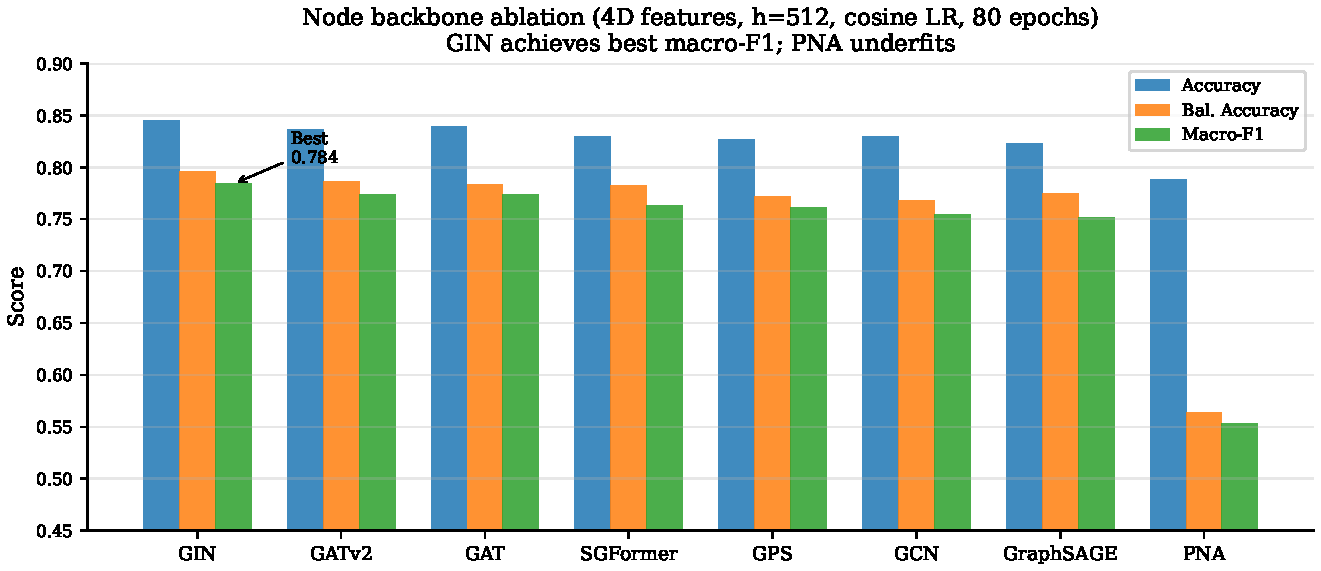
\includegraphics[width=\linewidth]{figures/backbone_ablation.pdf}
  \caption{Node backbone ablation: accuracy, balanced accuracy, and macro-F1
           for eight backbone types (4D features, all other hyperparameters fixed).}
  \label{fig:backbone_ablation}
\end{figure}

\subsection{Per-class Analysis}

The seven hardest classes --- 61, 90, 70, 56, 86, 14, 80 --- contribute
disproportionately to macro-F1 degradation.
Class\,80 achieves near-zero F1 in most configurations due to very few
training examples and high intra-class variability.
Classes 61 and 90 (the near-inseparable pair) produce complementary F1
scores: when the model predicts more class-61 samples correctly it
misclassifies more class-90, and vice versa
(F1 of 0.576 vs.\ 0.850 for the best run).

\subsection{Evaluation Protocol}
\label{sec:eval_protocol}

\paragraph{The 88-class vs.\ 99-class problem.}
The SHREC\,25 test set contains proteins from only \textbf{88 of the 99
families}: 11 families have training samples but zero test samples.
The model still outputs logits for all 99 classes at inference time.

When sklearn's \texttt{f1\_score(..., average='macro')} is called without
an explicit class list it includes every class appearing in the union of
ground-truth and prediction arrays.
Classes absent from the test set have support\,=\,0; their per-class F1 is
set to 0 by \texttt{zero\_division=0}.
The macro average then divides by 99 instead of 88:

\[
  \text{Macro-F1}_{99} = \frac{\sum_{c=0}^{87} F1_c +
    \underbrace{0 + \cdots + 0}_{11}}{99}
  = \frac{88}{99}\;\text{Macro-F1}_{88}
\]

This deflates the reported number by a factor of $88/99 \approx 0.889$
(e.g.\ $0.798 \rightarrow 0.710$ for the 8D model).

\paragraph{How we address it.}
All metrics in this report are computed by passing an explicit class list
to every sklearn metric call:

\begin{verbatim}
labels = sorted(valid_classes)   # 88 class IDs with >=1 test sample
f1_score(y_true, y_pred, average='macro',
         labels=labels, zero_division=0)
\end{verbatim}

This restricts the macro denominator to exactly 88, and classes with no
test samples are excluded from precision, recall, and F1.
Balanced accuracy is computed as macro-averaged recall over the same 88
class list.
Accuracy and weighted-F1 are unaffected (they weight by support, so
zero-support classes contribute nothing regardless).
